\ylDisplay{Must kast} % Ülesande nimi
{Kristian Kuppart} % Autor
{lõppvoor} % Voor
{2013} % Aasta
{G 4} % Ülesande nr.
{4} % Raskustase
{
% Teema: Elektriahelad
\ifStatement
\begin{wrapfigure}{r}{0.35\textwidth}%
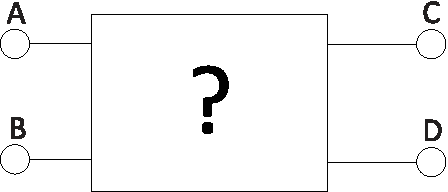
\includegraphics[width=\linewidth]{2013-v3g-04-pilt1}%
\end{wrapfigure}
Joonisel näidatud musta kasti kõik klemmid ühendatakse korraks kokku.
Seejärel, kui klemmide A ja B külge ühendada patarei
pingega $U$ ja klemmide C ja D külge voltmeeter, on voltmeetri näit alghetkel
$U$. Mõõtmise järel ühendatakse kõik klemmid veel korraks kokku.
Kui ühendada sama patarei klemmide C ja D külge ning voltmeeter
klemmide A ja B külge, on voltmeetri näit alghetkel~$\frac{U}{2}.$
Teades, et mustas kastis on ainult identsed kondensaatorid, joonistage musta kasti skeem.
\fi


\ifHint
Asjaolu, et voltmeeter näitab $\frac{U}{2}$, vihjab kondensaatorite jadaühendusele $C$ ja $D$ vahel.
\fi


\ifSolution
Sobiv skeem on näiteks selline:

\begin{center}
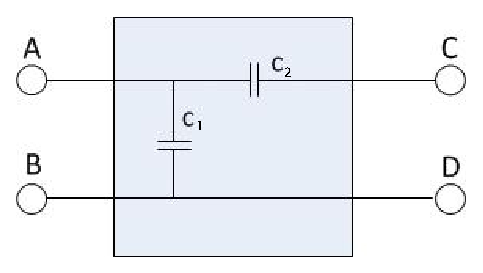
\includegraphics[width=0.5\textwidth]{2013-v3g-04-mustkastlah}\\
\end{center}

Kui klemmide A ja B külge ühendada patarei ja klemmide C ja D külge voltmeeter, siis läbi kondensaatori $C_2$ vool ei lähe ning ta ei laadu. Pinge temal on \num{0} ning voltmeeter näitab $U$.

Kui aga patarei ühendada klemmide C ja D külge ja voltmeeter klemmide A ja B külge, laaduvad mõlemad kondensaatorid üheaegselt ning pinge $U$ jaotub nende vahel võrdselt. Voltmeeter näitab $\frac{U}{2}$.
\fi


\ifEngStatement
% Problem name: Black box
\begin{wrapfigure}{r}{0.35\textwidth}%
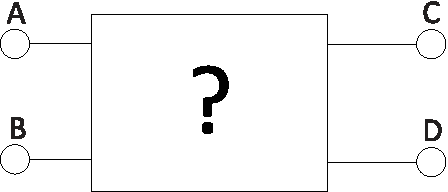
\includegraphics[width=\linewidth]{2013-v3g-04-pilt1}%
\end{wrapfigure}
All the black box’s leads given in the drawing are connected together for a moment. Next, if a battery of voltage $U$ is connected to the leads A and B and a voltmeter is connected with C and D then at the initial moment the voltmeter’s reading is $U$. After the measurement all the leads are connected together again. If the same battery is connected to the leads C and D and the voltmeter to the leads A and B the reading of the voltmeter is $\frac{U}{2}.$ at the initial moment. Knowing that there are only ideal capacitors in the black box, draw the circuit diagram of the black box.
\fi


\ifEngHint
The fact that the voltmeter shows $\frac{U}{2}$ hints that the capacitors are connected in series between $C$ and $D$.
\fi


\ifEngSolution
A suitable circuit can look like this:
\begin{center}
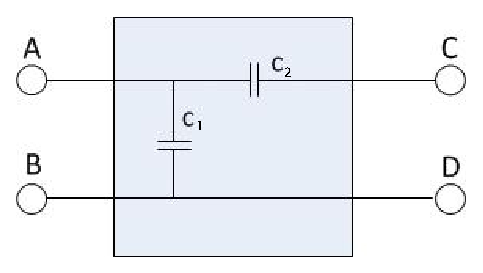
\includegraphics[width=0.5\textwidth]{2013-v3g-04-mustkastlah}\\
\end{center}
If a battery would be connected to the leads A and B and a voltmeter to the leads C and D then no current will go through the capacitor $C_2$ and it will not charge. The voltage on it is zero and the voltmeter’s reading is $U$.\\
However, if the battery would be connected to the leads C and D and the voltmeter to A and B then both of the capacitors will charge with the same time and the voltage $U$ will be divided equally between them. The voltmeter’s reading is $\frac{U}{2}$.
\fi
}